\section{Formalismo}
\label{Formalismo}

\noindent
La forma est�ndar en que se modelan los problemas de RL est� esquematizado en la figura~\ref{Fig:Formalismo}. En la figura se ve un robot que representa a un agente, y una nube gris que representa el ambiente. La interacci�n entre ambos es de la siguiente forma: en el instante $t$ el ambiente se encuentra en el estado $s_{t}$, y el agente recibe una observaci�n $i_{t}$, que depende de dicho estado. La funci�n $B$ es la que decide lo que el agente va a hacer, seleccionando una acci�n a tomar $a$. Luego de ejecutar dicha acci�n, el ambiente se encontrar� en un nuevo estado $s_{t+1}$, de acuerdo a una \textit{funci�n de transici�n} $T$, y produce una se�al de refuerzo $r$, que tambi�n es funci�n del estado $s_{t}$.

\subsection{Markov Decision Process}
\noindent
La interacci�n entre el agente y su ambiente suele formalizarse como Proceso de decisi�n de Markov (\textit{Markov Decision Process}, MDP en adelante). Un MDP es una tupla $\mathcal{M} = \langle \mathcal{S}, \mathcal{A}, \mathcal{T}, \mathcal{R}, \gamma \rangle$, donde:
\begin{itemize}
 \item $\mathcal{S}$ es el conjunto de estados en el que se puede encontrar el ambiente. Puede ser discreto o continuo.
 \item $\mathcal{A}$ es el conjunto de acciones a disposici�n del agente. Puede ser discreto o continuo.
 \item $T(s,a,s')$ representa la probabilidad de pasar al estado $s'$ estando en el estado $s$ y ejecutando la acci�n $a$.
 \item $R(s,a)$ indica el refuerzo esperado de ejecutar $a$ en $s$.
 \item $\gamma \in (0,1]$ es el \textit{factor de descuento}. Una interpretaci�n usual es que $\gamma$ representa ``la probabilidad de seguir vivo en el pr�ximo instante''. La idea es que si esta probabilidad es menor que 1, refuerzos que espero obtener en el futuro ``valen'' menos que los que espero obtener pr�ximamente, porque en el futuro quiz�s ya ni est� vivo.
\end{itemize}

\begin{figure}[h!]
\centering
\includegraphics[scale=1.1]{imagen/rl_model}
\caption{Modelo RL estandar}
\label{Fig:Formalismo}
\end{figure}


\subsection{Pol�tica}
\noindent
Un agente elige sus acciones de acuerdo a una pol�tica (\textit{policy}). Formalmente, una pol�tica es una funci�n $\pi: \mathcal{S} \rightarrow \mathcal{A}$. Es decir, dado un estado $s$, $\pi(s)$ nos devuelve la acci�n a tomar desde el estado $s$.

